\documentclass[12pt]{article}
\usepackage{diagbox}

%%%%%%%%%%%%%%%%%%%%%%%%%%%%%%%%%%%%%%%%%
% Lachaise Assignment
% Structure Specification File
% Version 1.0 (26/6/2018)
%
% This template originates from:
% http://www.LaTeXTemplates.com
%
% Authors:
% Marion Lachaise & François Févotte
% Vel (vel@LaTeXTemplates.com)
%
% License:
% CC BY-NC-SA 3.0 (http://creativecommons.org/licenses/by-nc-sa/3.0/)
% 
%%%%%%%%%%%%%%%%%%%%%%%%%%%%%%%%%%%%%%%%%

%----------------------------------------------------------------------------------------
%	PACKAGES AND OTHER DOCUMENT CONFIGURATIONS
%----------------------------------------------------------------------------------------

\usepackage{amsmath,amsfonts,stmaryrd,amssymb} % Math packages

\usepackage{enumerate} % Custom item numbers for enumerations

\usepackage[ruled]{algorithm2e} % Algorithms

\usepackage[framemethod=tikz]{mdframed} % Allows defining custom boxed/framed environments

\usepackage{listings} % File listings, with syntax highlighting
\lstset{
	basicstyle=\ttfamily, % Typeset listings in monospace font
}

%----------------------------------------------------------------------------------------
%	DOCUMENT MARGINS
%----------------------------------------------------------------------------------------

\usepackage{geometry} % Required for adjusting page dimensions and margins

\geometry{
	paper=a4paper, % Paper size, change to letterpaper for US letter size
	top=2.5cm, % Top margin
	bottom=3cm, % Bottom margin
	left=2.5cm, % Left margin
	right=2.5cm, % Right margin
	headheight=14pt, % Header height
	footskip=1.5cm, % Space from the bottom margin to the baseline of the footer
	headsep=1.2cm, % Space from the top margin to the baseline of the header
	%showframe, % Uncomment to show how the type block is set on the page
}

%----------------------------------------------------------------------------------------
%	FONTS
%----------------------------------------------------------------------------------------

\usepackage[utf8]{inputenc} % Required for inputting international characters
\usepackage[T1]{fontenc} % Output font encoding for international characters

\usepackage{XCharter} % Use the XCharter fonts

%----------------------------------------------------------------------------------------
%	COMMAND LINE ENVIRONMENT
%----------------------------------------------------------------------------------------

% Usage:
% \begin{commandline}
%	\begin{verbatim}
%		$ ls
%		
%		Applications	Desktop	...
%	\end{verbatim}
% \end{commandline}

\mdfdefinestyle{commandline}{
	leftmargin=10pt,
	rightmargin=10pt,
	innerleftmargin=15pt,
	middlelinecolor=black!50!white,
	middlelinewidth=2pt,
	frametitlerule=false,
	backgroundcolor=black!5!white,
	frametitle={Command Line},
	frametitlefont={\normalfont\sffamily\color{white}\hspace{-1em}},
	frametitlebackgroundcolor=black!50!white,
	nobreak,
}

% Define a custom environment for command-line snapshots
\newenvironment{commandline}{
	\medskip
	\begin{mdframed}[style=commandline]
}{
	\end{mdframed}
	\medskip
}

%----------------------------------------------------------------------------------------
%	FILE CONTENTS ENVIRONMENT
%----------------------------------------------------------------------------------------

% Usage:
% \begin{file}[optional filename, defaults to "File"]
%	File contents, for example, with a listings environment
% \end{file}

\mdfdefinestyle{file}{
	innertopmargin=1.6\baselineskip,
	innerbottommargin=0.8\baselineskip,
	topline=false, bottomline=false,
	leftline=false, rightline=false,
	leftmargin=2cm,
	rightmargin=2cm,
	singleextra={%
		\draw[fill=black!10!white](P)++(0,-1.2em)rectangle(P-|O);
		\node[anchor=north west]
		at(P-|O){\ttfamily\mdfilename};
		%
		\def\l{3em}
		\draw(O-|P)++(-\l,0)--++(\l,\l)--(P)--(P-|O)--(O)--cycle;
		\draw(O-|P)++(-\l,0)--++(0,\l)--++(\l,0);
	},
	nobreak,
}

% Define a custom environment for file contents
\newenvironment{file}[1][File]{ % Set the default filename to "File"
	\medskip
	\newcommand{\mdfilename}{#1}
	\begin{mdframed}[style=file]
}{
	\end{mdframed}
	\medskip
}

%----------------------------------------------------------------------------------------
%	NUMBERED QUESTIONS ENVIRONMENT
%----------------------------------------------------------------------------------------

% Usage:
% \begin{question}[optional title]
%	Question contents
% \end{question}

\mdfdefinestyle{question}{
	innertopmargin=1.2\baselineskip,
	innerbottommargin=0.8\baselineskip,
	roundcorner=5pt,
	nobreak,
	singleextra={%
		\draw(P-|O)node[xshift=1em,anchor=west,fill=white,draw,rounded corners=5pt]{%
		Question \theQuestion\questionTitle};
	},
}

\newcounter{Question} % Stores the current question number that gets iterated with each new question

% Define a custom environment for numbered questions
\newenvironment{question}[1][\unskip]{
	\bigskip
	\stepcounter{Question}
	\newcommand{\questionTitle}{~#1}
	\begin{mdframed}[style=question]
}{
	\end{mdframed}
	\medskip
}

%----------------------------------------------------------------------------------------
%	WARNING TEXT ENVIRONMENT
%----------------------------------------------------------------------------------------

% Usage:
% \begin{warn}[optional title, defaults to "Warning:"]
%	Contents
% \end{warn}

\mdfdefinestyle{warning}{
	topline=false, bottomline=false,
	leftline=false, rightline=false,
	nobreak,
	singleextra={%
		\draw(P-|O)++(-0.5em,0)node(tmp1){};
		\draw(P-|O)++(0.5em,0)node(tmp2){};
		\fill[black,rotate around={45:(P-|O)}](tmp1)rectangle(tmp2);
		\node at(P-|O){\color{white}\scriptsize\bf !};
		\draw[very thick](P-|O)++(0,-1em)--(O);%--(O-|P);
	}
}

% Define a custom environment for warning text
\newenvironment{warn}[1][Warning:]{ % Set the default warning to "Warning:"
	\medskip
	\begin{mdframed}[style=warning]
		\noindent{\textbf{#1}}
}{
	\end{mdframed}
}

%----------------------------------------------------------------------------------------
%	INFORMATION ENVIRONMENT
%----------------------------------------------------------------------------------------

% Usage:
% \begin{info}[optional title, defaults to "Info:"]
% 	contents
% 	\end{info}

\mdfdefinestyle{info}{%
	topline=false, bottomline=false,
	leftline=false, rightline=false,
	nobreak,
	singleextra={%
		\fill[black](P-|O)circle[radius=0.4em];
		\node at(P-|O){\color{white}\scriptsize\bf i};
		\draw[very thick](P-|O)++(0,-0.8em)--(O);%--(O-|P);
	}
}

% Define a custom environment for information
\newenvironment{info}[1][Info:]{ % Set the default title to "Info:"
	\medskip
	\begin{mdframed}[style=info]
		\noindent{\textbf{#1}}
}{
	\end{mdframed}
}

\title{VE527: Assignment \#5} % Title of the assignment
\author{Name: Chang Meng\\Student ID:\@\texttt{118370910019}}
\date{}

\begin{document}

    \maketitle
    \noindent
    1. (10\%) What is the function $F(a, b, c)$ for the following ROBDD\@?
    \begin{center}
        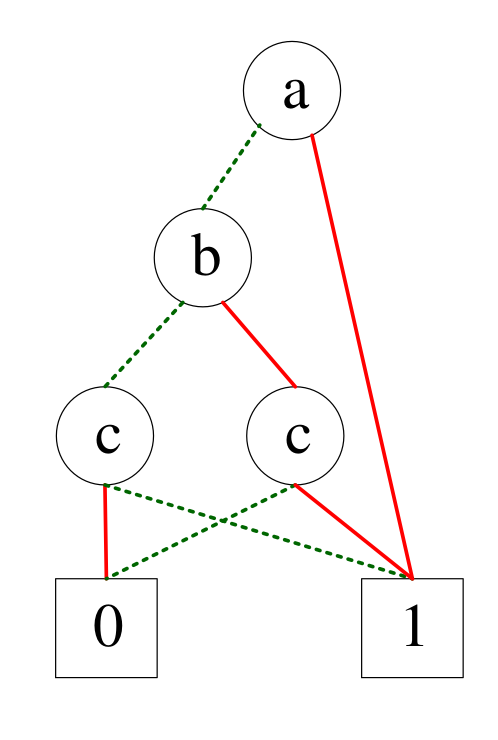
\includegraphics[width = 1.50in, height = 2.20in]{figure1.png}
    \end{center}

    \noindent
    Answer:

    \noindent
    There are 3 paths from $a$ to $0$:
    $a$,
    $\bar{a}bc$,
    and $\bar{a}\bar{b}\bar{c}$.
    So the function is:
    \[
        F(a, b, c) = a + \bar{a}bc + \bar{a}\bar{b}\bar{c} = a + \bar{b}\bar{c} + bc
    \]

    \noindent
    2. (10\%) How many input patterns $(a, b, c, d)$,
    where $a, b, c, d \in {0, 1}$,
    will satisfy the following BDD (i.e., let the function of this BDD be 1)?

    \begin{center}
        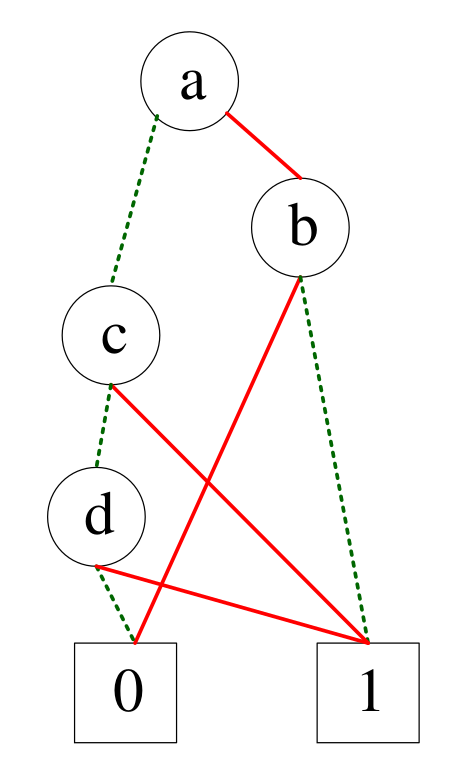
\includegraphics[width = 1.50in, height = 2.20in]{figure2.png}
    \end{center}

    \noindent
    Answer:

    \noindent
    There are 10 input patterns.
    They are (1, 0, 0, 0), (1, 0, 0, 1), (1, 0, 1, 0), (1, 0, 1, 1),
    (0, 0, 1, 0), (0, 0, 1, 1), (0, 1, 1, 0), (0, 1, 1, 1),
    (0, 0, 0, 1), (0, 1, 0, 1).

    \noindent
    3. (40\%) A simple comparator takes two 2-bit unsigned binary numbers $a_{1}a_{0}$ and $b_{1}b_{0}$ and compares their maginitude.
    Its output $Z = 1$ if and only if $a_{1}a_{0}$ is GREATER THAN $b_{1}b_{0}$.
    For example,
    since $a_{1}a_{0} = 11 > b_{1}b_{0} = 01$,
    the output $Z = 1$.
    However,
    for $a_{1}a_{0} = 01$ and $b_{1}b_{0} = 01$,
    since they are equal,
    the output $Z = 0$.

    \noindent
    Draw the ROBDD for the output Z of the 2-bit comparator.
    Suppose the variable ordering is $b_{0} < a_{0} < b_{1} < a_{1}$ (i.e., $b_{0}$ is the closest to the root and $a_{1}$ is the farest away from the root).
    What does the ROBDD look like for the variable ordering $a_{1} < b_{1} < a_{0} < b_{0}$?

    \noindent
    Answer:

    \noindent
    All possible patterns for $Z = 1$ are listed below:
    \begin{center}
        \begin{tabular}{|c|c|}
            \hline
            $a_{1}a_{0}$ & $b_{1}b_{0}$ that is smaller than $a_{1}a_{0}$ \\
            \hline
            $00$ & $\verb|\|$ \\
            \hline
            $01$ & $00$ \\
            \hline
            $10$ & $00, 01$ \\
            \hline
            $11$ & $00, 01, 10$ \\
            \hline
        \end{tabular}
    \end{center}
    The K-Map is shown below:
    \begin{center}
        \begin{tabular}{|c|c|c|c|c|c|}
            \hline
            \diagbox{$b_{1}b_{0}$}{$a_{1}a_{0}$} & 00 & 01 & 11 & 10 \\
            \hline
            00 & 0 & 1 & 1 & 1 \\
            \hline
            01 & 0 & 0 & 1 & 1 \\
            \hline
            11 & 0 & 0 & 0 & 0 \\
            \hline
            10 & 0 & 0 & 1 & 0 \\
            \hline
        \end{tabular}
    \end{center}
    So $Z = a_{1}\bar{b_{1}} + a_{1}a_{0}\bar{b_{0}} + a_{0}\bar{b_{1}}\bar{b_{0}}$.

    \noindent
    In the ordering of $b_{0} < a_{0} < b_{1} < a_{1}$,
    I decompose $Z$ recursively:\\
    $b_{0}$:\\
    $Z_{b_{0}} = a_{1}\bar{b_{1}}$, $Z_{\bar{b_{0}}} = a_{1}\bar{b_{1}} + a_{1}a_{0} + a_{0}\bar{b_{1}}$;\\
    $a_{0}$:\\
    $Z_{b_{0}}$ is not relevant to $a_{0}$;\\
    $Z_{\bar{b_{0}}a_{0}} = a_{1}\bar{b_{1}} + a_{1} + \bar{b_{1}} = a_{1} + \bar{b_{1}} $,
    $Z_{\bar{b_{0}}\bar{a_{0}}} = a_{1}\bar{b_{1}}$;\\
    $b_{1}$:\\
    $Z_{b_{0}b_{1}} = 0$, $Z_{b_{0}\bar{b_{1}}} = a_{1}$;\\
    $Z_{\bar{b_{0}}a_{0}b_{1}} = a_{1}$,
    $Z_{\bar{b_{0}}a_{0}\bar{b_{1}}} = 1$;\\
    $Z_{\bar{b_{0}}\bar{a_{0}}b_{1}} = 0$,
    $Z_{\bar{b_{0}}\bar{a_{0}}\bar{b_{1}}} = a_{1}$.\\

    \begin{center}
        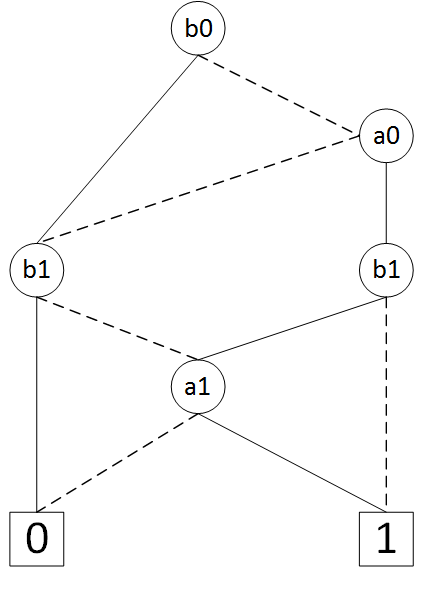
\includegraphics[width = 2.00in, height = 2.50in]{figure4.png}
    \end{center}

    \noindent
    In the ordering of $a_{1} < b_{1} < a_{0} < b_{0}$,
    I decompose $Z$ recursively:\\
    $a_{1}$:\\
    $Z_{a_{1}} = \bar{b_{1}} + a_{0}\bar{b_{0}} + a_{0}\bar{b_{1}}\bar{b_{0}} = \bar{b_{1}} + a_{0}\bar{b_{0}}$,
    $Z_{\bar{a_{1}}} = a_{0}\bar{b_{1}}\bar{b_{0}}$;\\
    $b_{1}$:\\
    $Z_{a_{1}b_{1}} = a_{0}\bar{b_{0}}$,
    $Z_{a_{1}\bar{b_{1}}} = 1$;\\
    $Z_{\bar{a_{1}}b_{1}} = 0$,
    $Z_{\bar{a_{1}}\bar{b_{1}}} = a_{0}\bar{b_{0}}$;\\
    $a_{0}$:\\
    $Z_{a_{1}b_{1}a_{0}} = \bar{b_{0}}$,
    $Z_{a_{1}b_{1}\bar{a_{0}}} = 0$;\\
    $Z_{\bar{a_{1}}\bar{b_{1}}a_{0}} = \bar{b_{0}}$,
    $Z_{\bar{a_{1}}\bar{b_{1}}\bar{a_{0}}} = 0$.\\

    \begin{center}
        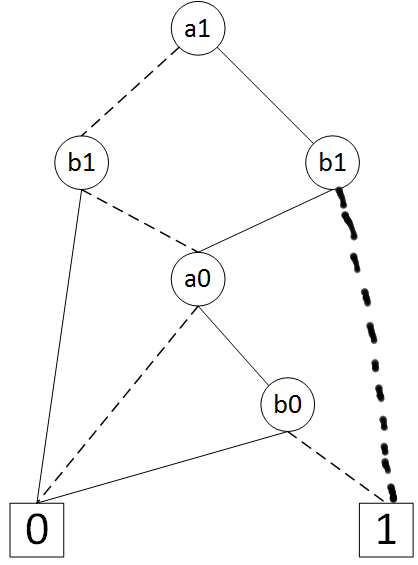
\includegraphics[width = 2.00in, height = 2.50in]{figure5.png}
    \end{center}

    \noindent
    4. (18\%) Consider the function $f$ expressed in the CNF form:
    \[
        f = \omega_{1}\omega_{2}\dots\omega_{8}
    \]
    where $\omega_{1} = a_{1} + a_{2}$,
    $\omega_{2} = a_{1} + a_{2} + a_{3} + \bar{a_{4}}$,
    $\omega_{3} = \bar{a_{2}} + a_{4}$,
    $\omega_{4} = a_{1} + \bar{a_{2}} + \bar{a_{4}}$,
    $\omega_{5} = \bar{a_{1}} + a_{2} + a_{4}$,
    $\omega_{6} = \bar{a_{1}} + a_{2} + a_{3}$,
    $\omega_{7} = \bar{a_{1}} + \bar{a_{2}} + \bar{a_{4}} + \bar{a_5}$,
    $\omega_{8} = \bar{a_{1}} + a_{2} + \bar{a_{3}} + a_{4} + \bar{a_5}$.

    \noindent
    Assume that we have decide $a_{4} = 0$.
    Make this assignment and then run Boolean constraint propagation (BCP) by applying the unit clause rule.
    You should continue BCP \underline{until} you cannot make any additional progress on the formula.
    What is your conclusion after BCP and simplification?
    If the CNF is still unresolved, show the final CNF\@.

    \noindent
    Answer:

    \noindent
    Applying $a_{4} = 0$:\\
    $\omega_{1} = a_{1} + a_{2}$,\\
    $\omega_{2} = 1$,\\
    $\omega_{3} = \bar{a_{2}}$,\\
    $\omega_{4} = 1$,\\
    $\omega_{5} = \bar{a_{1}} + a_{2}$;\\
    $\omega_{6} = \bar{a_{1}} + a_{2} + a_{3}$,\\
    $\omega_{7} = 1$,\\
    $\omega_{8} = \bar{a_{1}} + a_{2} + \bar{a_{3}} + \bar{a_5}$.\\
    Implicate $a_{2} = 0$:\\
    $\omega_{1} = a_{1}$,\\
    $\omega_{2} = 1$,\\
    $\omega_{3} = 1$,\\
    $\omega_{4} = 1$,\\
    $\omega_{5} = \bar{a_{1}}$;\\
    $\omega_{6} = \bar{a_{1}} + a_{3}$,\\
    $\omega_{7} = 1$,\\
    $\omega_{8} = \bar{a_{1}} + \bar{a_{3}} + \bar{a_5}$.\\
    Implicate $a_{1} = 1$ from $\omega_{1} = a_{1}$:\\
    $\omega_{1} = 1$,\\
    $\omega_{2} = 1$,\\
    $\omega_{3} = 1$,\\
    $\omega_{4} = 1$,\\
    $\omega_{5} = 0$;\\
    $\omega_{6} = a_{3}$,\\
    $\omega_{7} = 1$,\\
    $\omega_{8} = \bar{a_{3}} + \bar{a_5}$.\\
    $\omega{5}$ is conficting.\\
    The conclusion is that there does not exist a SAT assignment for $a_{4} = 0$,
    then $a_{4} = 1$ should be tried.

    \noindent
    5. (10\%) BDDs operating on general Boolean logic,
    and SAT solvers operating on CNF clause lists,
    are both techniques that we can use to work with complex logic.
    But they each have different capabilities.
    Which of the following statements are true about each respective technology?
    Select the correct ones.
    \begin{enumerate}[a)]
        \item
            We can use a BDD to find ALL satisfying assignemnts of a Boolean function.
        \item
            We can use SAT to find a satisfying assignment of a Boolean function.
        \item
            SAT solvers and BDD packages may not always work for any Boolean function.
        \item
            SAT solvers and BDD packages will always work for any Boolean function.
        \item
            We can use a BDD to find a satisfying assignment of a Boolean function.
        \item
            A SAT solver allows us to perform many manipulations on a set of Boolean functions,
            such as AND, OR, NOT, XOR, XNOR, ect.
        \item
            A BDD package allows us to perform many manipulations on a set of Boolean functions,
            such as AND, OR, NOT, XOR, XNOR, ect.
        \item
            Suppose we have two gate level hardware implementations of some functions,
            call them F and G.
            We want to check if the hardware for F produces identical outputs as the hardware for G.
            We can do this using BDDs,
            but we cannot do this using a SAT solver.
        \item
            Suppose we have two gate level hardware implementations of some functions,
            call them F and G.
            We want to check if the hardware for F produces identical outputs as the hardware for G.
            We can do this using a SAT solver,
            but we cannot do this using BDDs.

    \end{enumerate}

    \noindent
    Answer:

    \noindent
    a), b), c), e), g) are correct.

    \noindent
    6. (12\%) As we talked in lecture,
    we can apply SAT to check if two different gate-level implementations $F$ and $G$ of a logic function are identical.
    In this problem,
    we will try a trivial example.
    We want to compare wheter $F(x, y) = x$ is identical to $G(x, y) = x + xy$.
    The figure below shows the gate-level circuit on which we can ask the SAT question to see whether $F$ and $G$ are identical.
    We have also leabled two internal nodes as $p$ and $q$ as shown below.
    Write the CNF formula that is satisfiable if and only if the gate-level circuit below is satisfiable.
    \begin{center}
        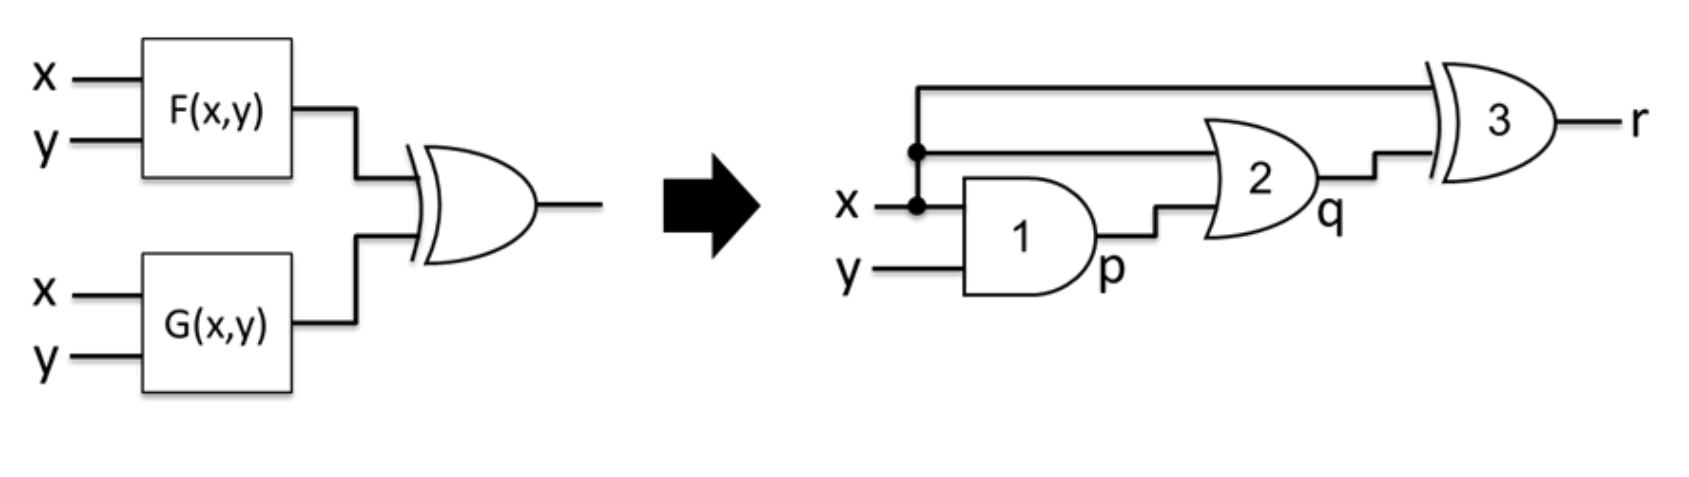
\includegraphics[width = 6.50in, height = 1.80in]{figure3.png}
    \end{center}

    \noindent
    \underline{Hint}: apply the gate consistency function discucssed in class.

    \noindent
    Answer:

    \noindent
    $\Phi_{p} = (x + \bar{p})(y + \bar{p})(\bar{x} + \bar{y} + p)$,\\
    $\Phi_{q} = (\bar{x} + q)(\bar{p} + q)(x + p + \bar{q})$,\\
    $\Phi_{r} = (\bar{x} + \bar{q} + \bar{r})(x + q + \bar{r})(x + \bar{q} + r)(\bar{x} + q + r)$.\\
    $\Psi = r\Phi_{p}\Phi_{q}\Phi_{r}=r(x + \bar{p})(y + \bar{p})(\bar{x} + \bar{y} + p)(\bar{x} + q)(\bar{p} + q)(x + p + \bar{q})(\bar{x} + \bar{q} + \bar{r})(x + q + \bar{r})(x + \bar{q} + r)(\bar{x} + q + r)$.\\


\end{document}
